\subsubsection*{(e) \textbf{(1,0 pontos)}}
\textit{E assim por diante, repita os ítens (a) e (b) para 256, 512 e 1024 amostras do sinal.}

\textbf{Para 256 Amostras}

\begin{figure}[H]
    \centering
    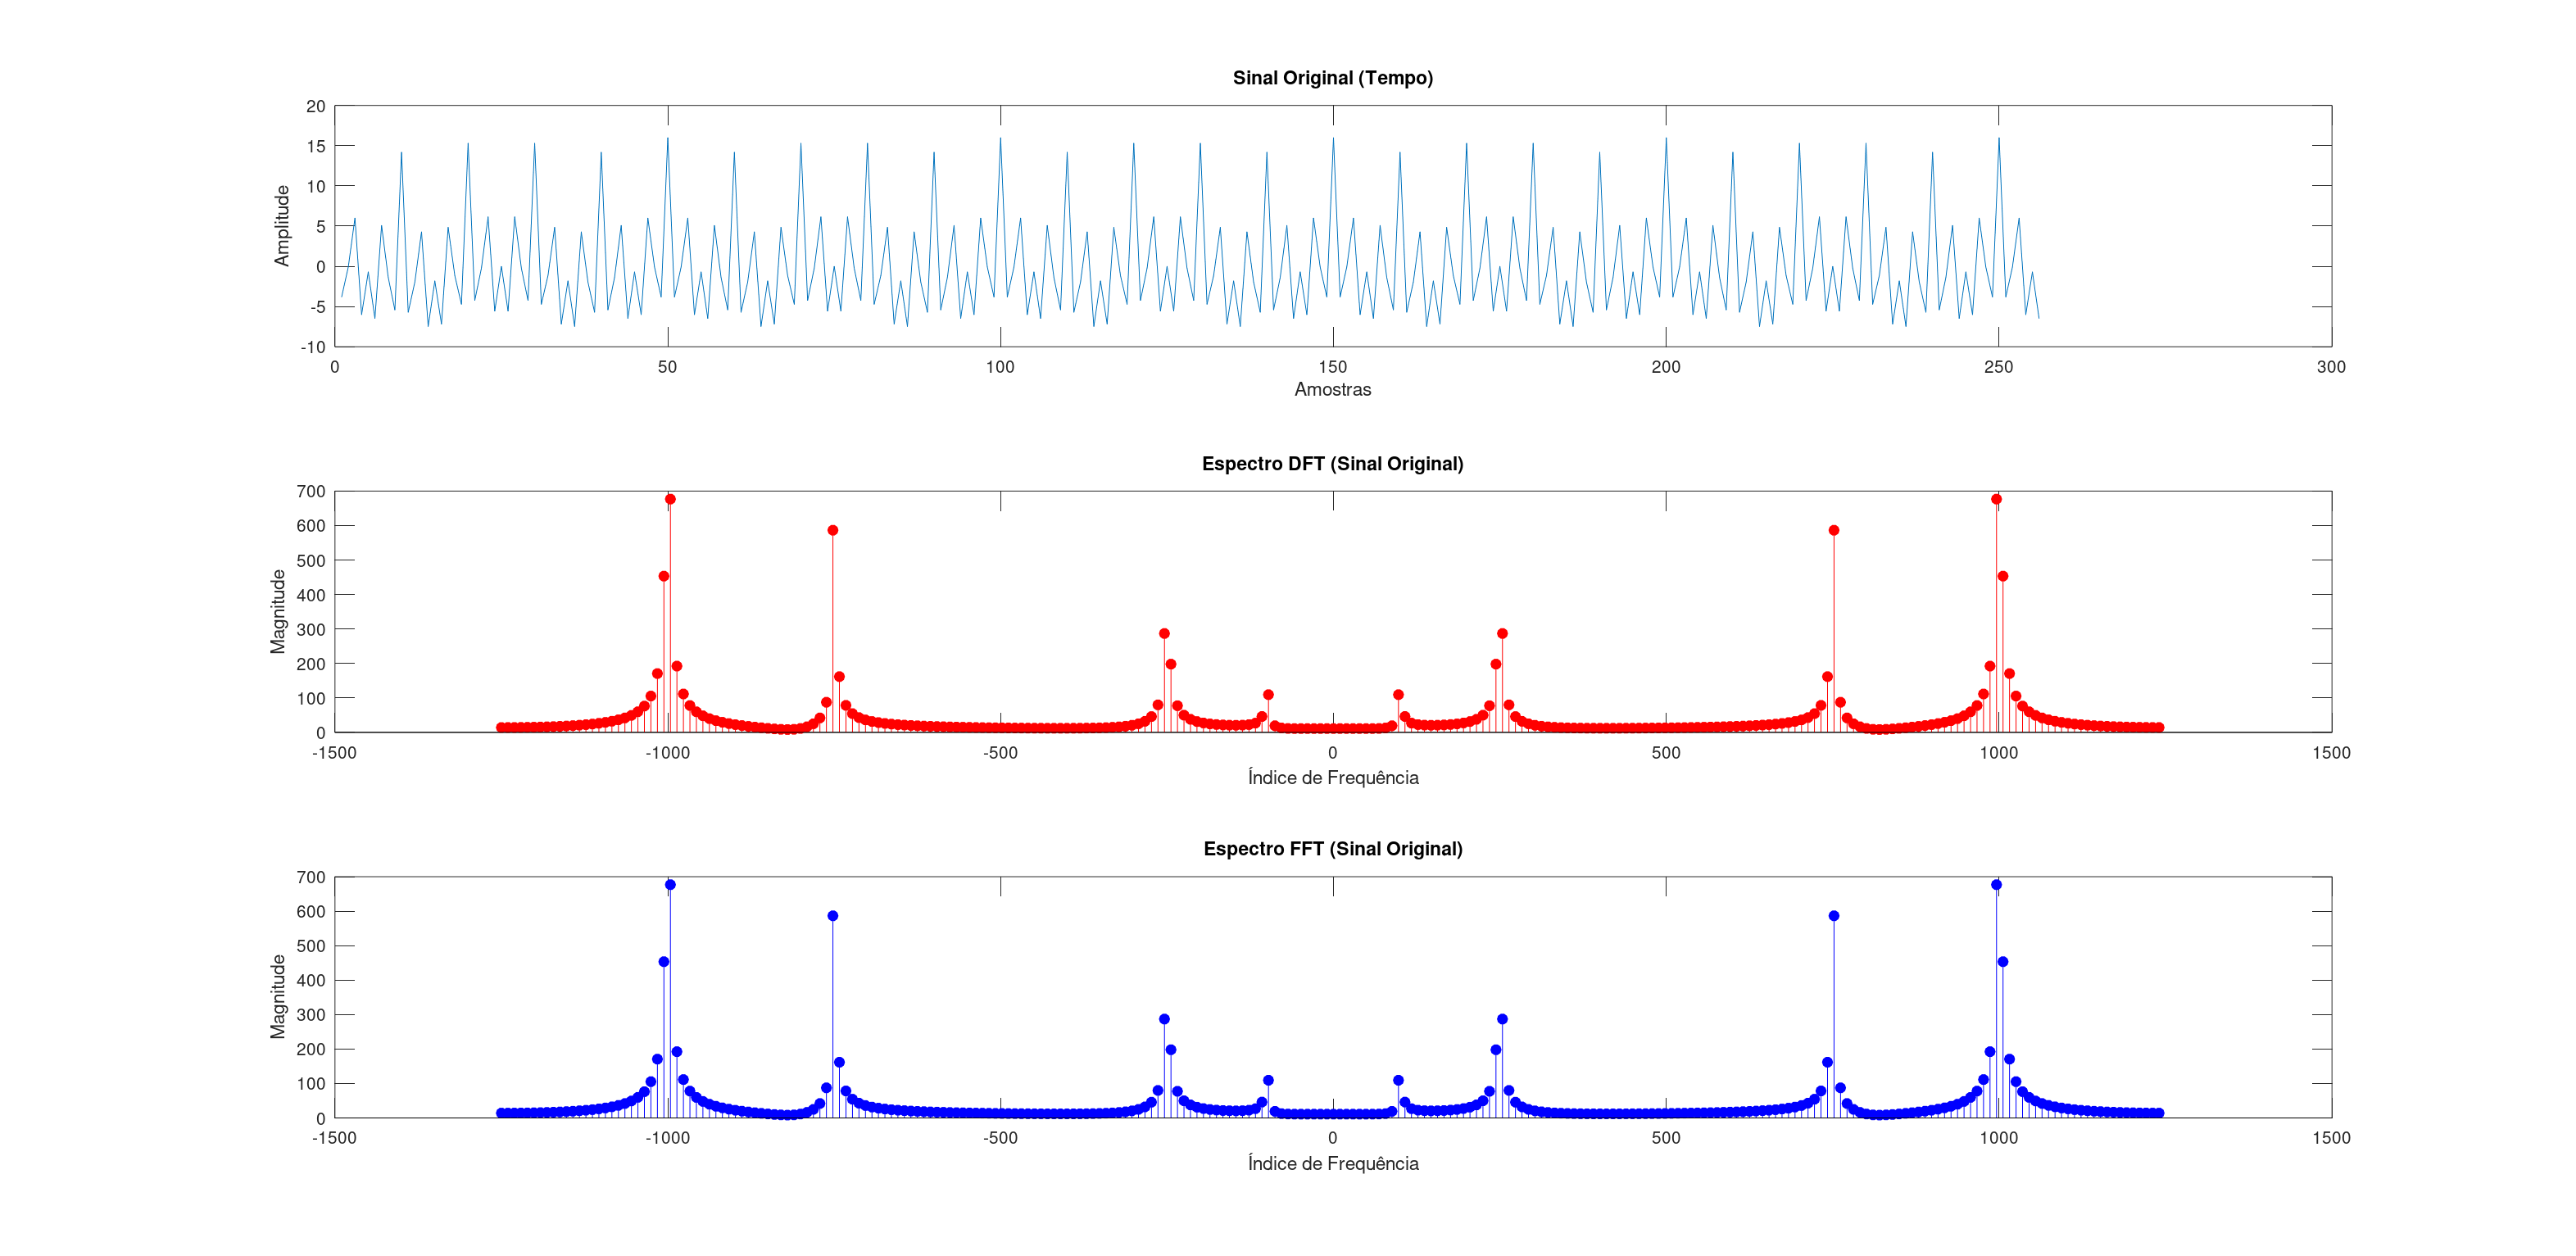
\includegraphics[width=1\linewidth]{03_experimental_analysis//assets/plot_results/256_samples_dft_fft.png}
    \caption{DFT+FFT Aplicada a 256 amostras}
    \label{fig:signal_256samples_fft-dft}
\end{figure}

\begin{figure}[H]
    \centering
    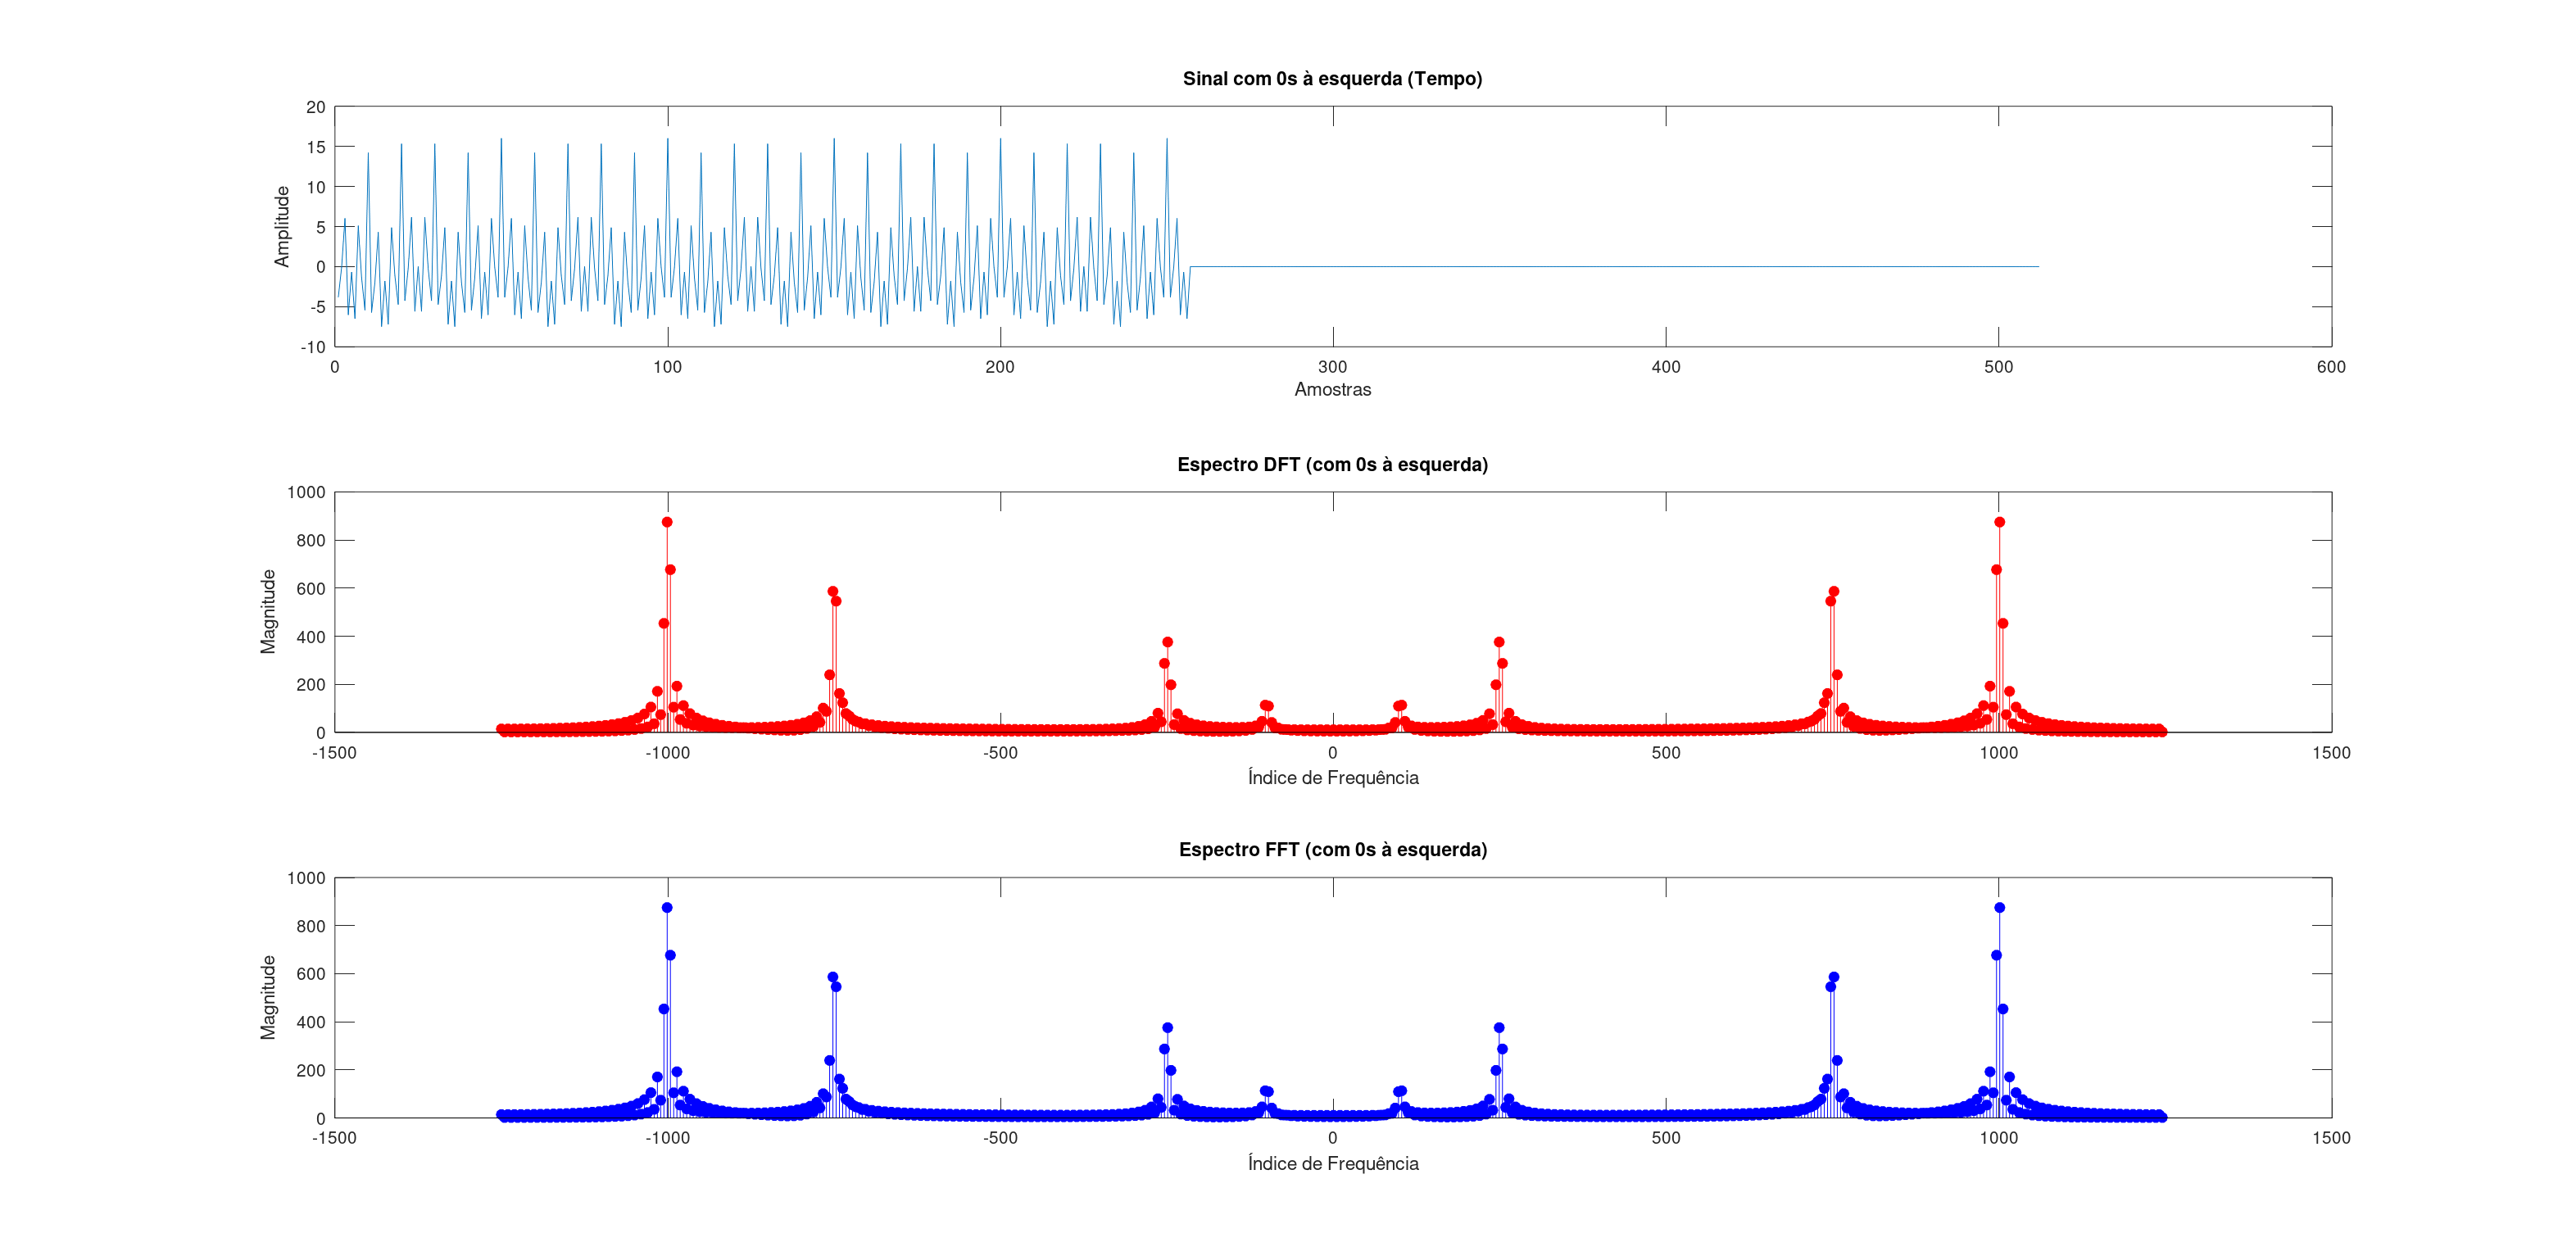
\includegraphics[width=1\linewidth]{03_experimental_analysis//assets/plot_results/256_samples_dft_fft_padded.png}
    \caption{DFT+FFT Aplicada a 256 amostras com 256 zeros à direita}
    \label{fig:signal_256samples_fft-dft_padded}
\end{figure}

%%%%%%%%%%%%%%%%%%%%%%%%%%%%%%%%%%%%%%%%%%%%%%%%%%%%%%%%%%%%%%%%%%%%
\textbf{Para 512 Amostras}

\begin{figure}[H]
    \centering
    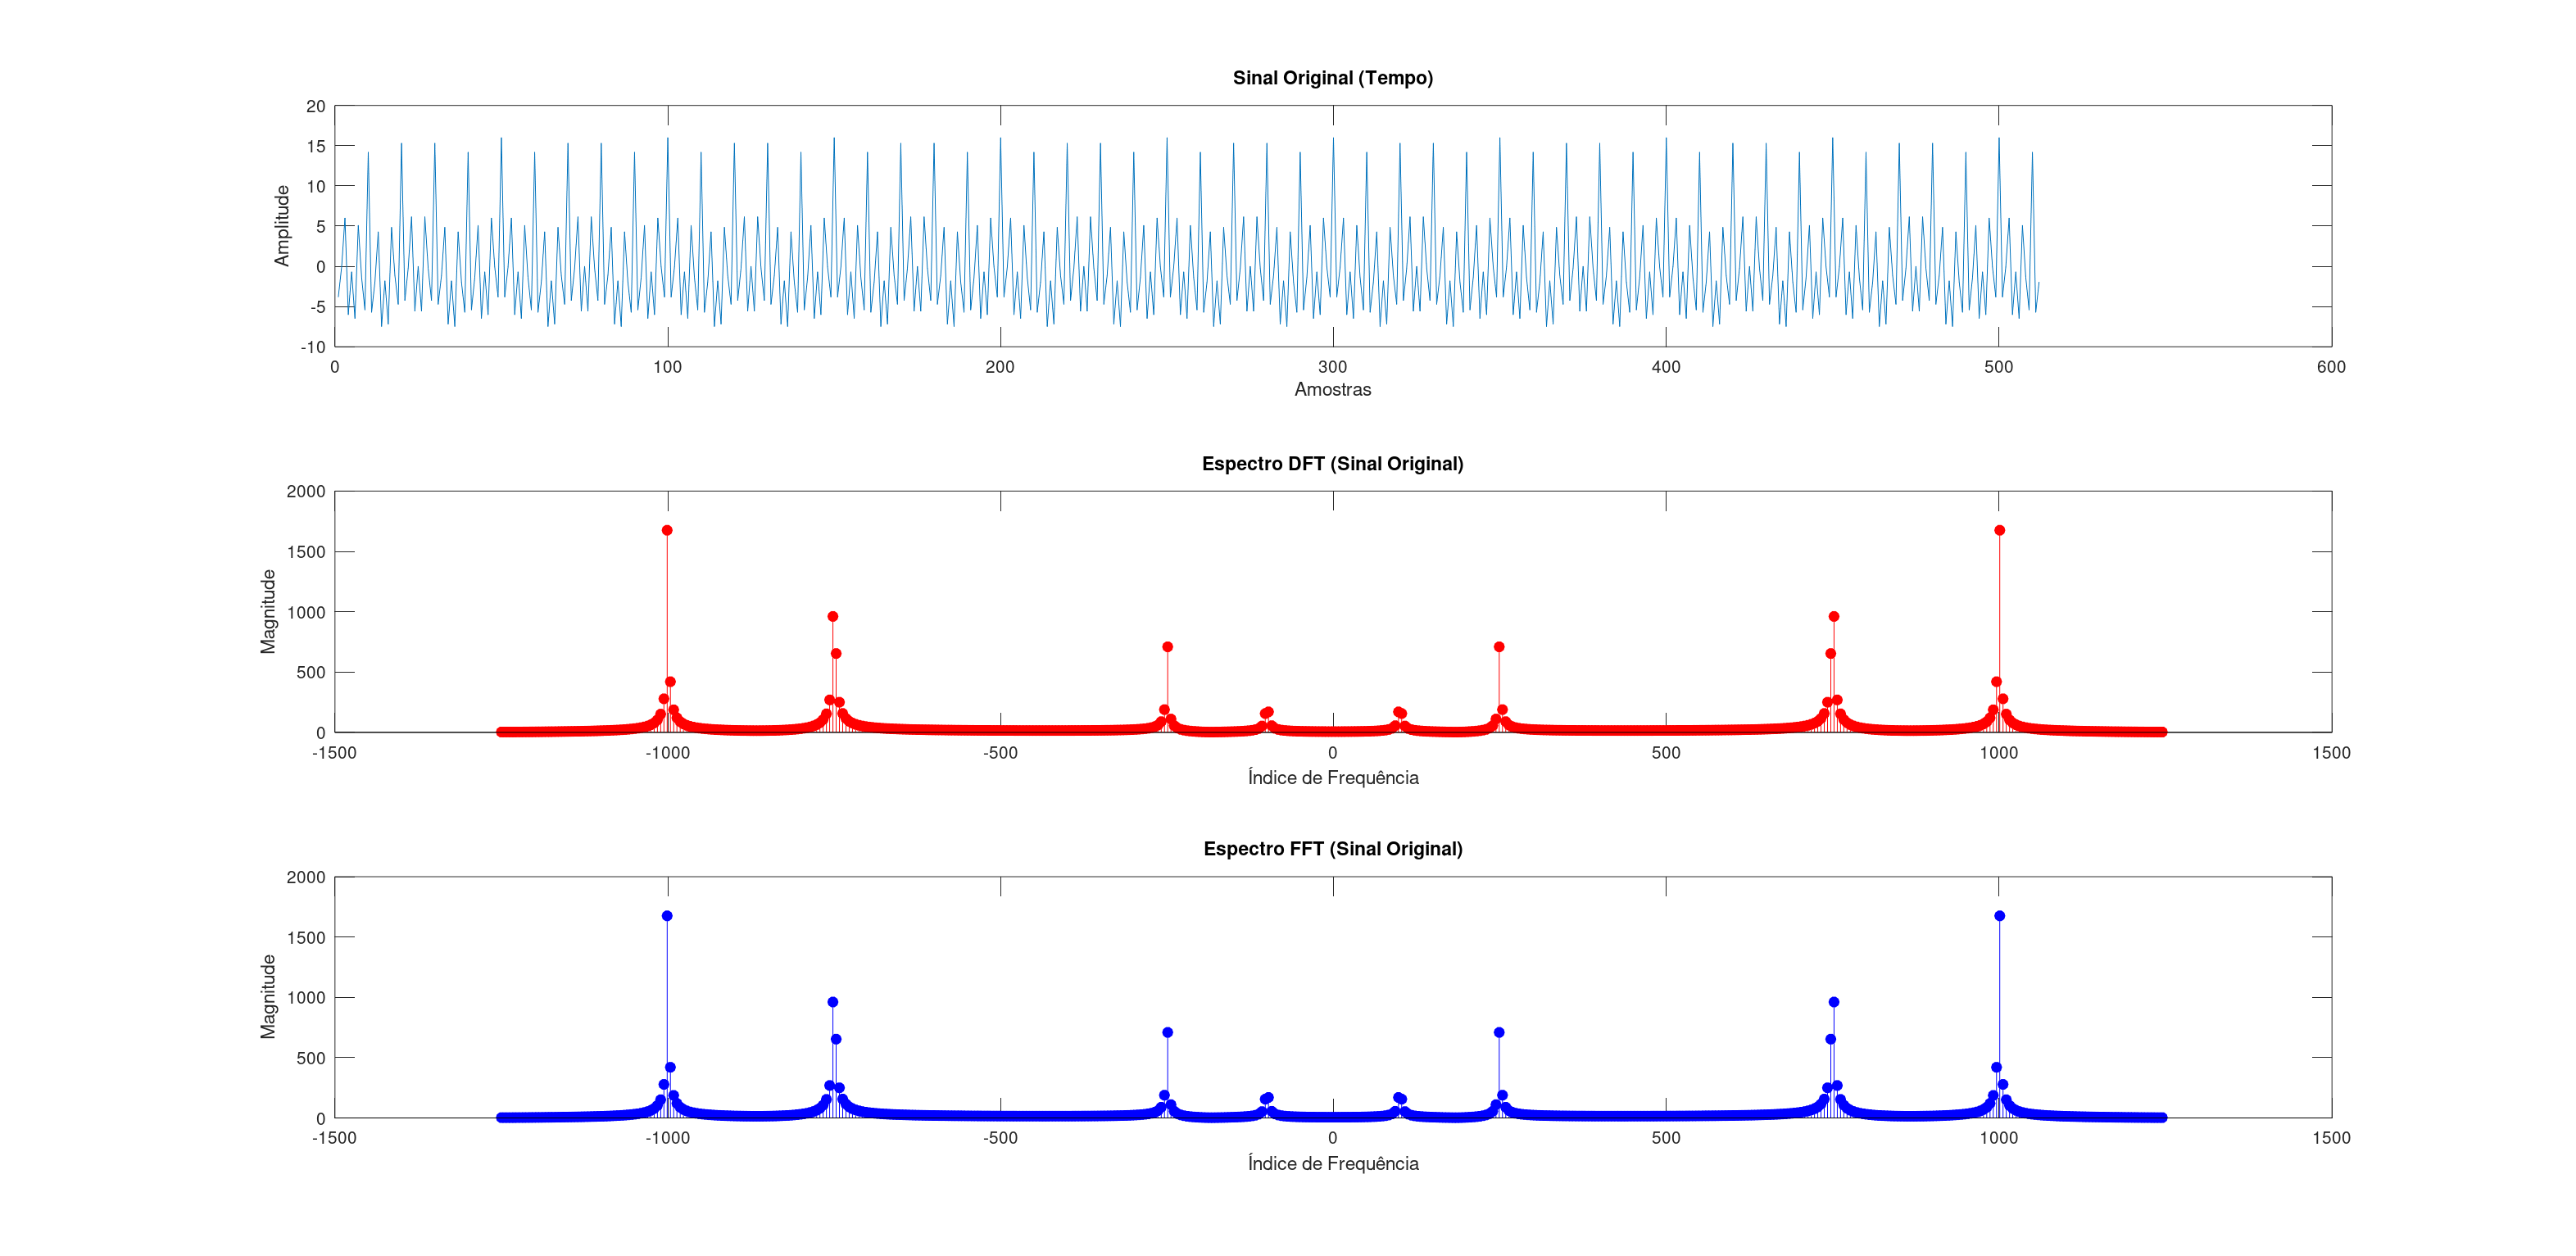
\includegraphics[width=1\linewidth]{03_experimental_analysis//assets/plot_results/512_samples_dft_fft.png}
    \caption{DFT+FFT Aplicada a 512 amostras}
    \label{fig:signal_512samples_fft-dft}
\end{figure}

\begin{figure}[H]
    \centering
    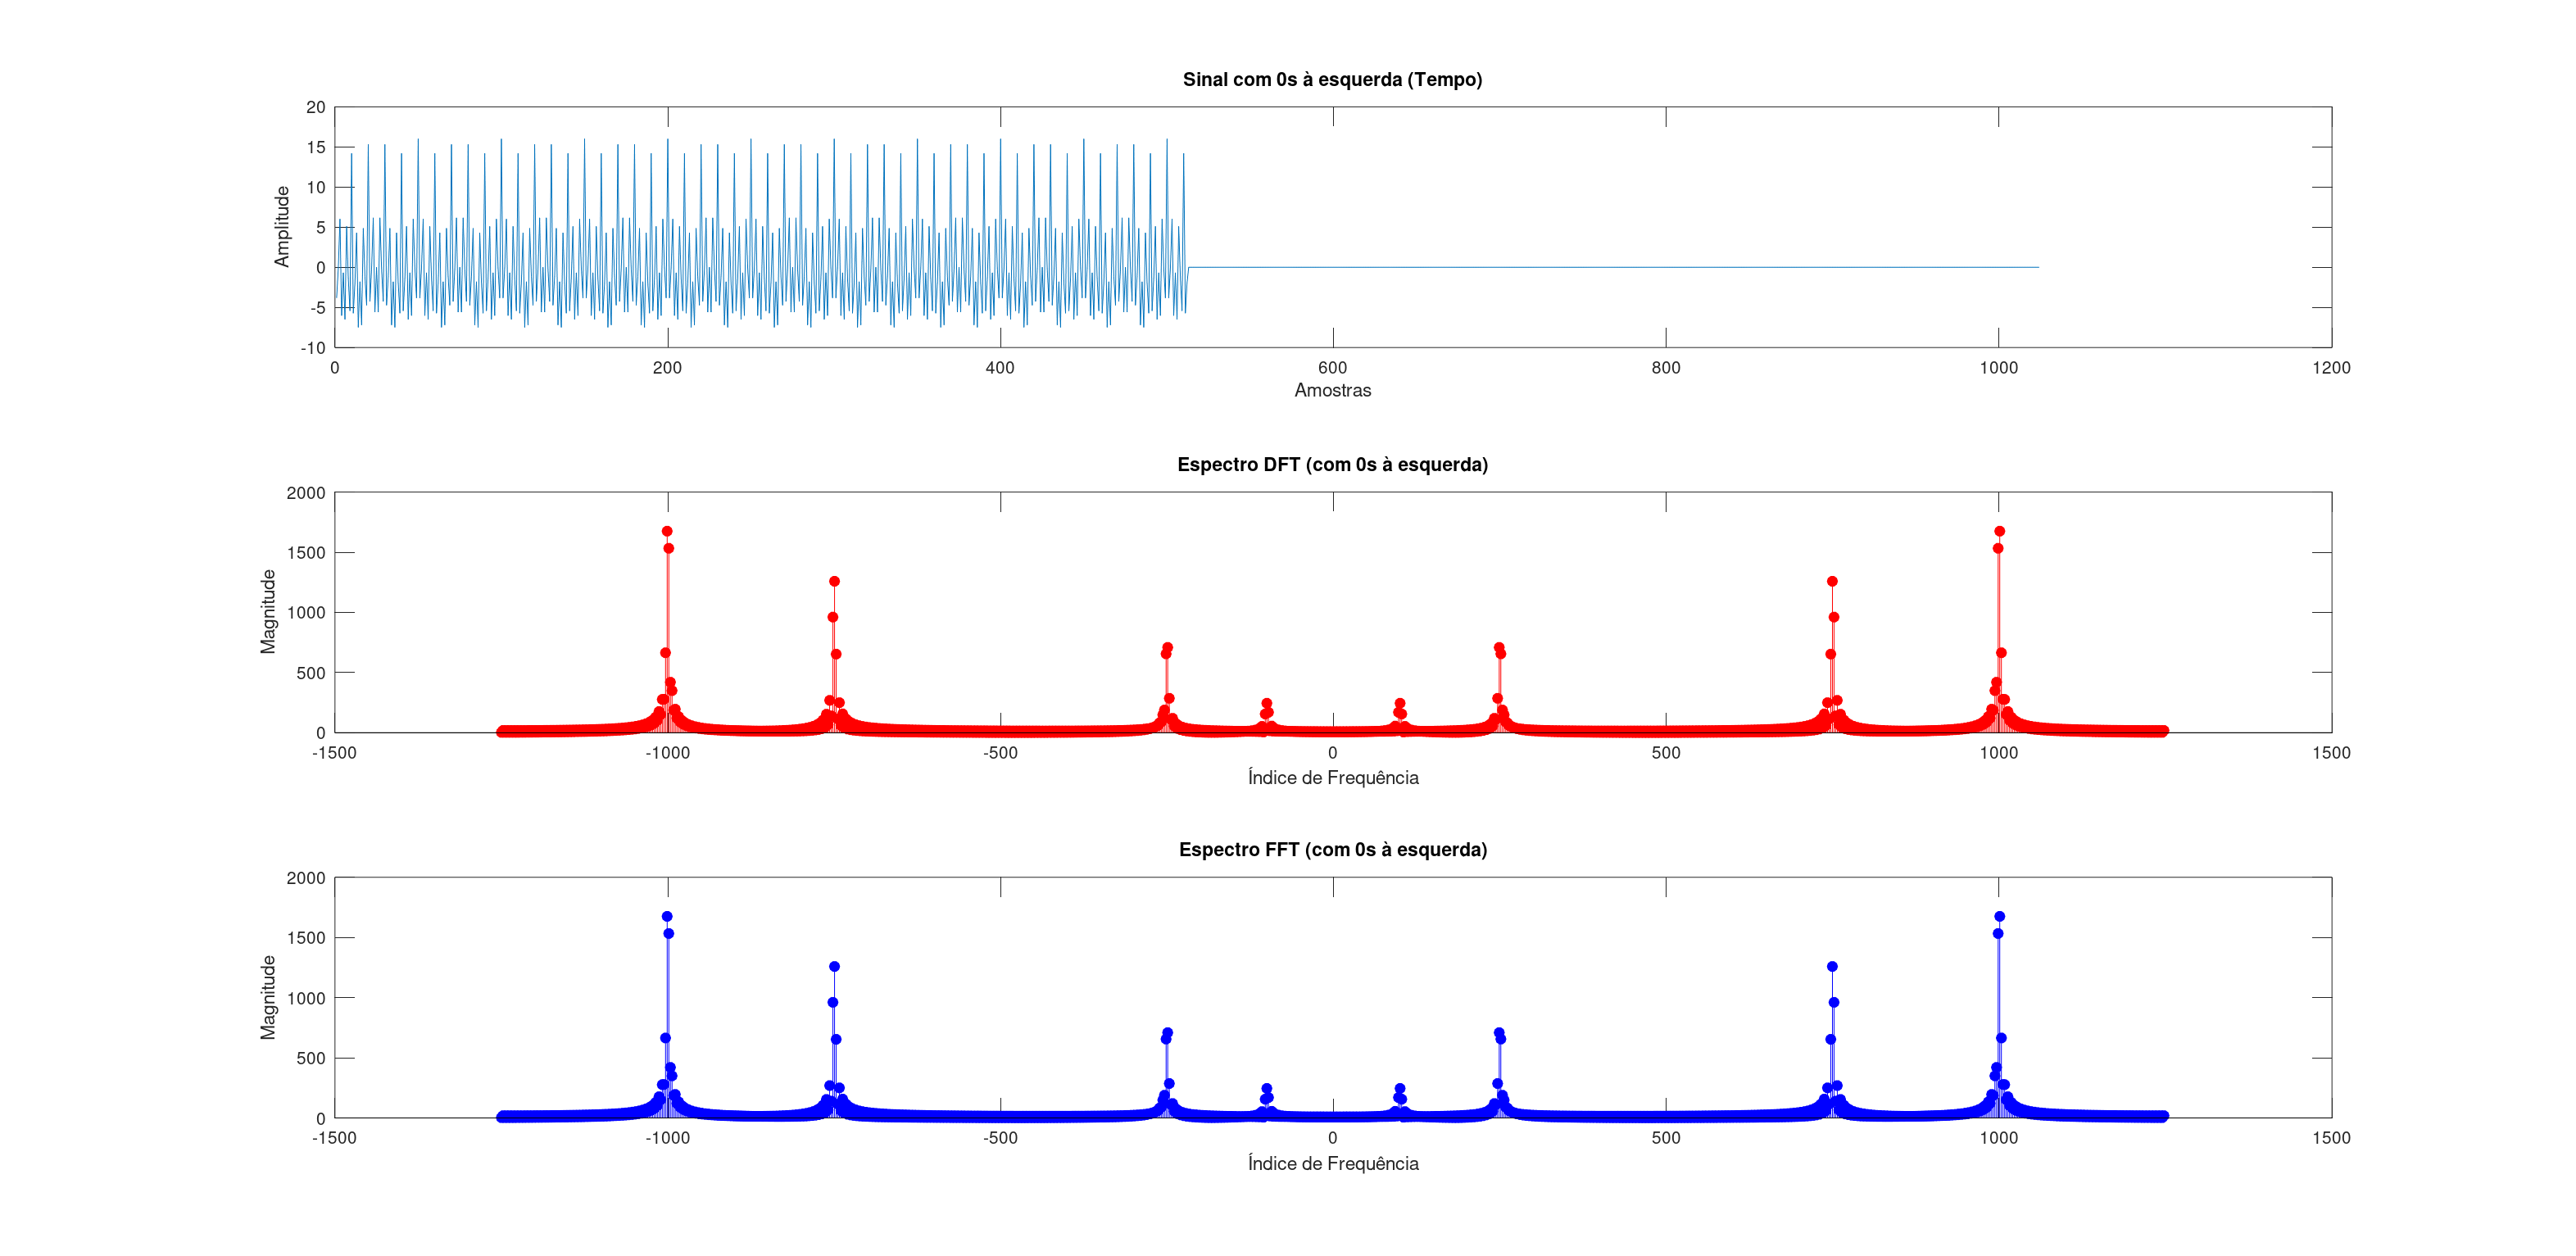
\includegraphics[width=1\linewidth]{03_experimental_analysis//assets/plot_results/512_samples_dft_fft_padded.png}
    \caption{DFT+FFT Aplicada a 512 amostras com 512 zeros à direita}
    \label{fig:signal_512samples_fft-dft_padded}
\end{figure}

%%%%%%%%%%%%%%%%%%%%%%%%%%%%%%%%%%%%%%%%%%%%%%%%%%%%%%%%%%%%%%%%%%%%
\textbf{Para 1024 Amostras}

\begin{figure}[H]
    \centering
    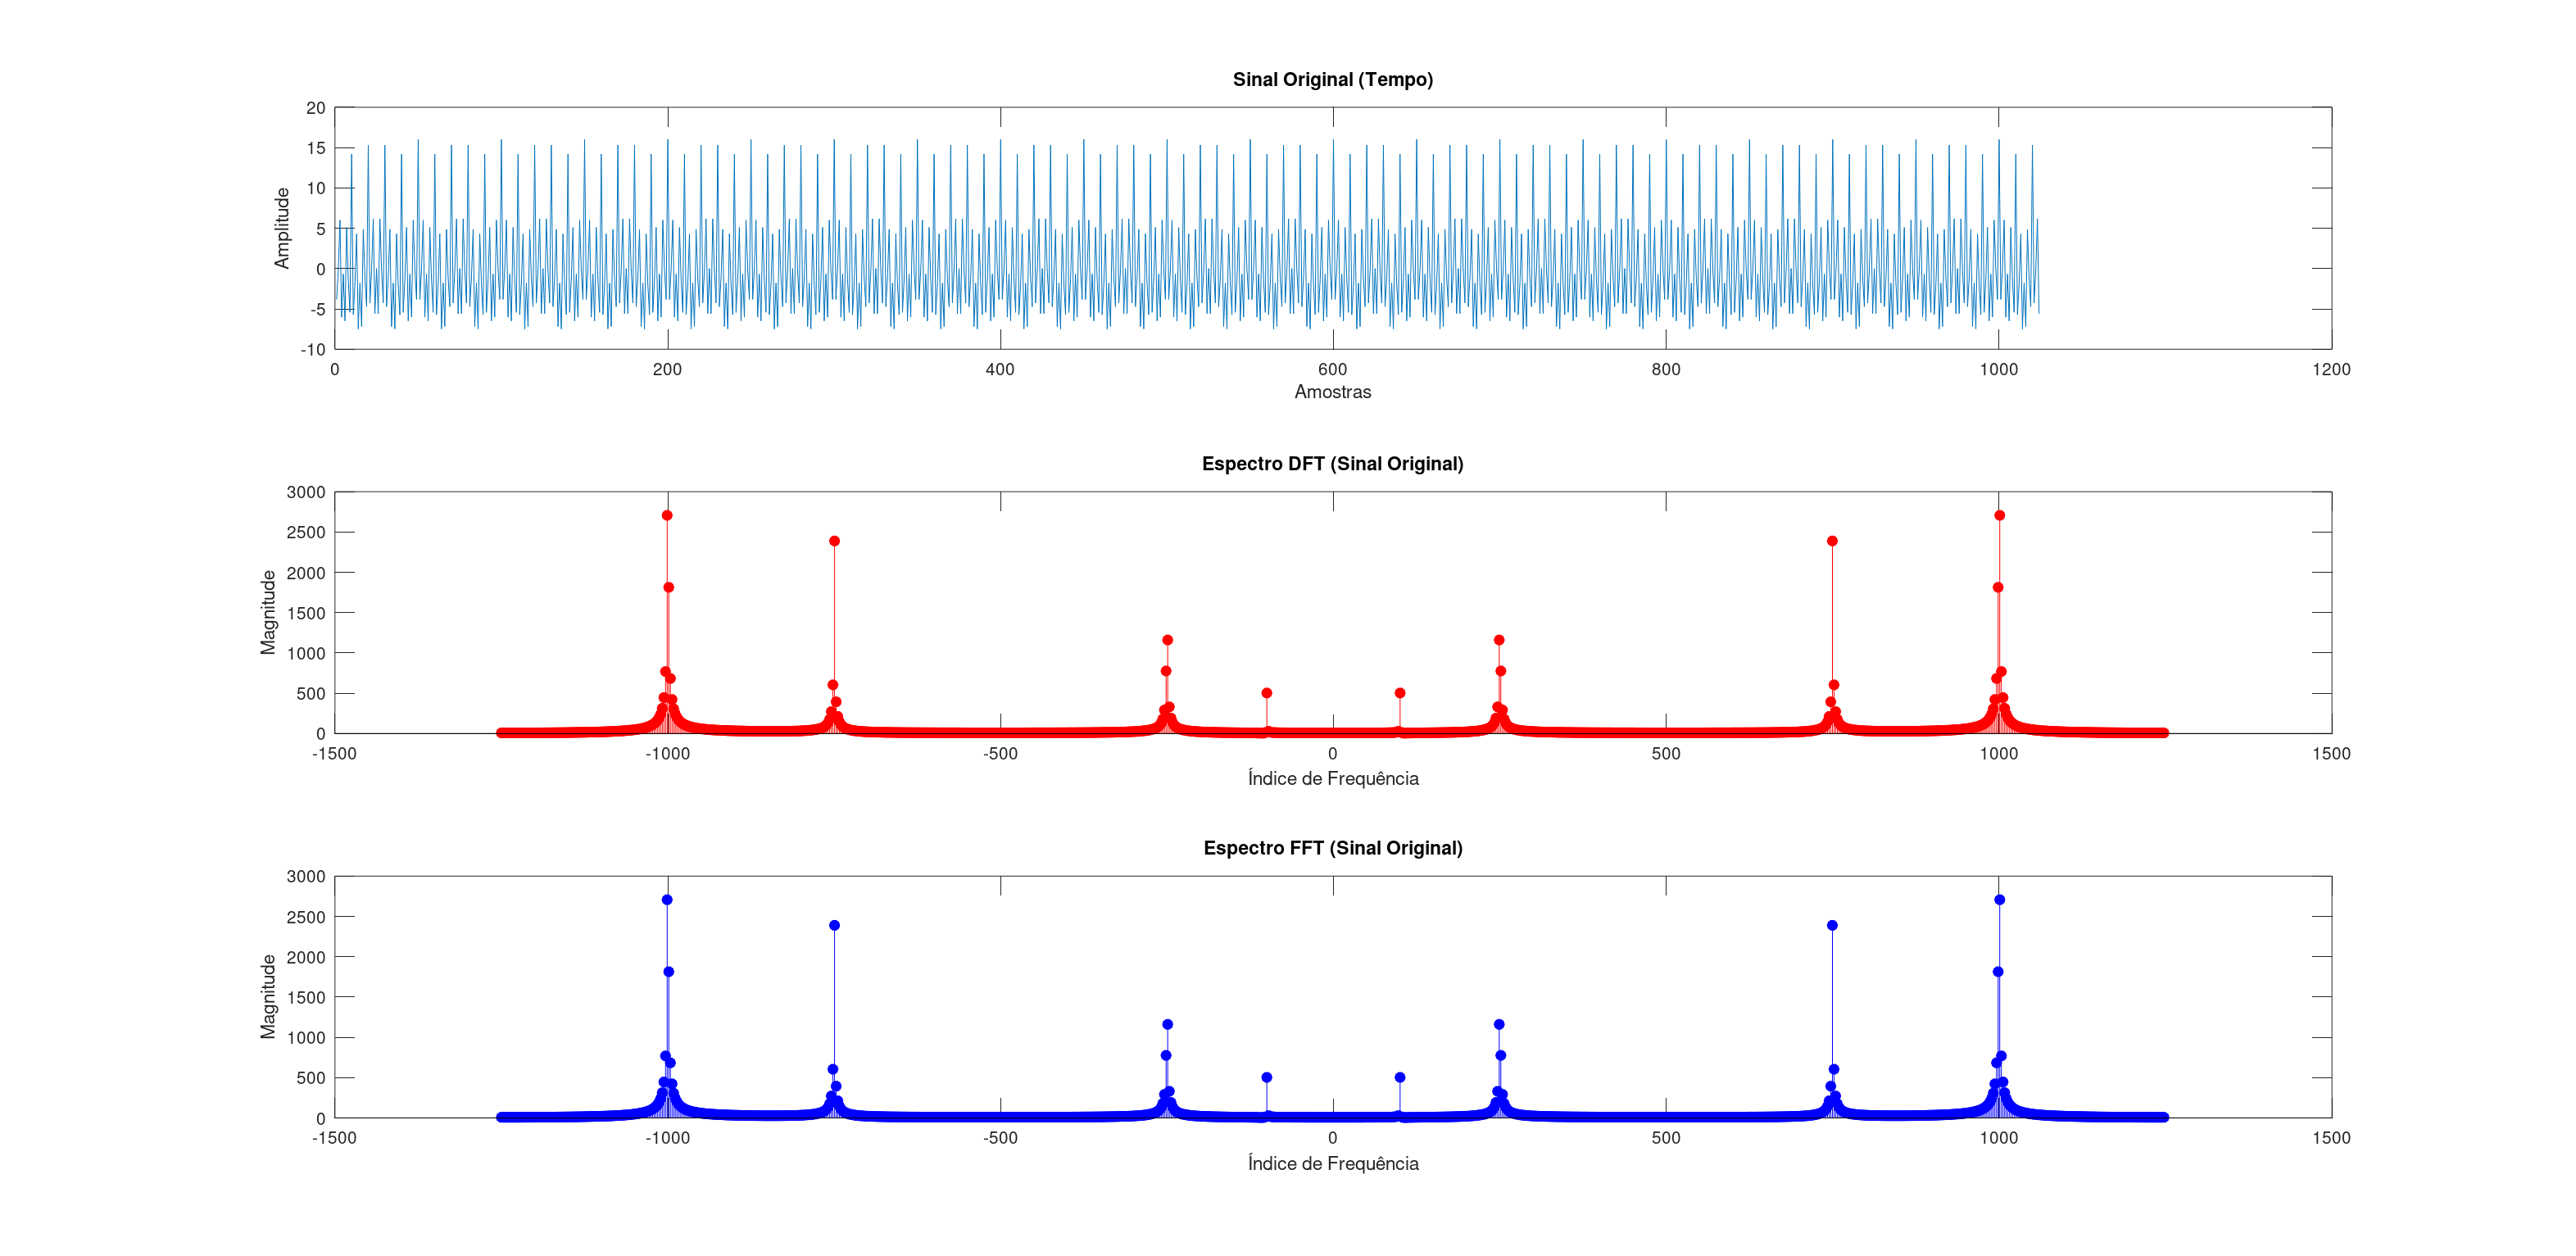
\includegraphics[width=1\linewidth]{03_experimental_analysis//assets/plot_results/1024_samples_dft_fft.png}
    \caption{DFT+FFT Aplicada a 1024 amostras}
    \label{fig:signal_1024samples_fft-dft}
\end{figure}

\begin{figure}[H]
    \centering
    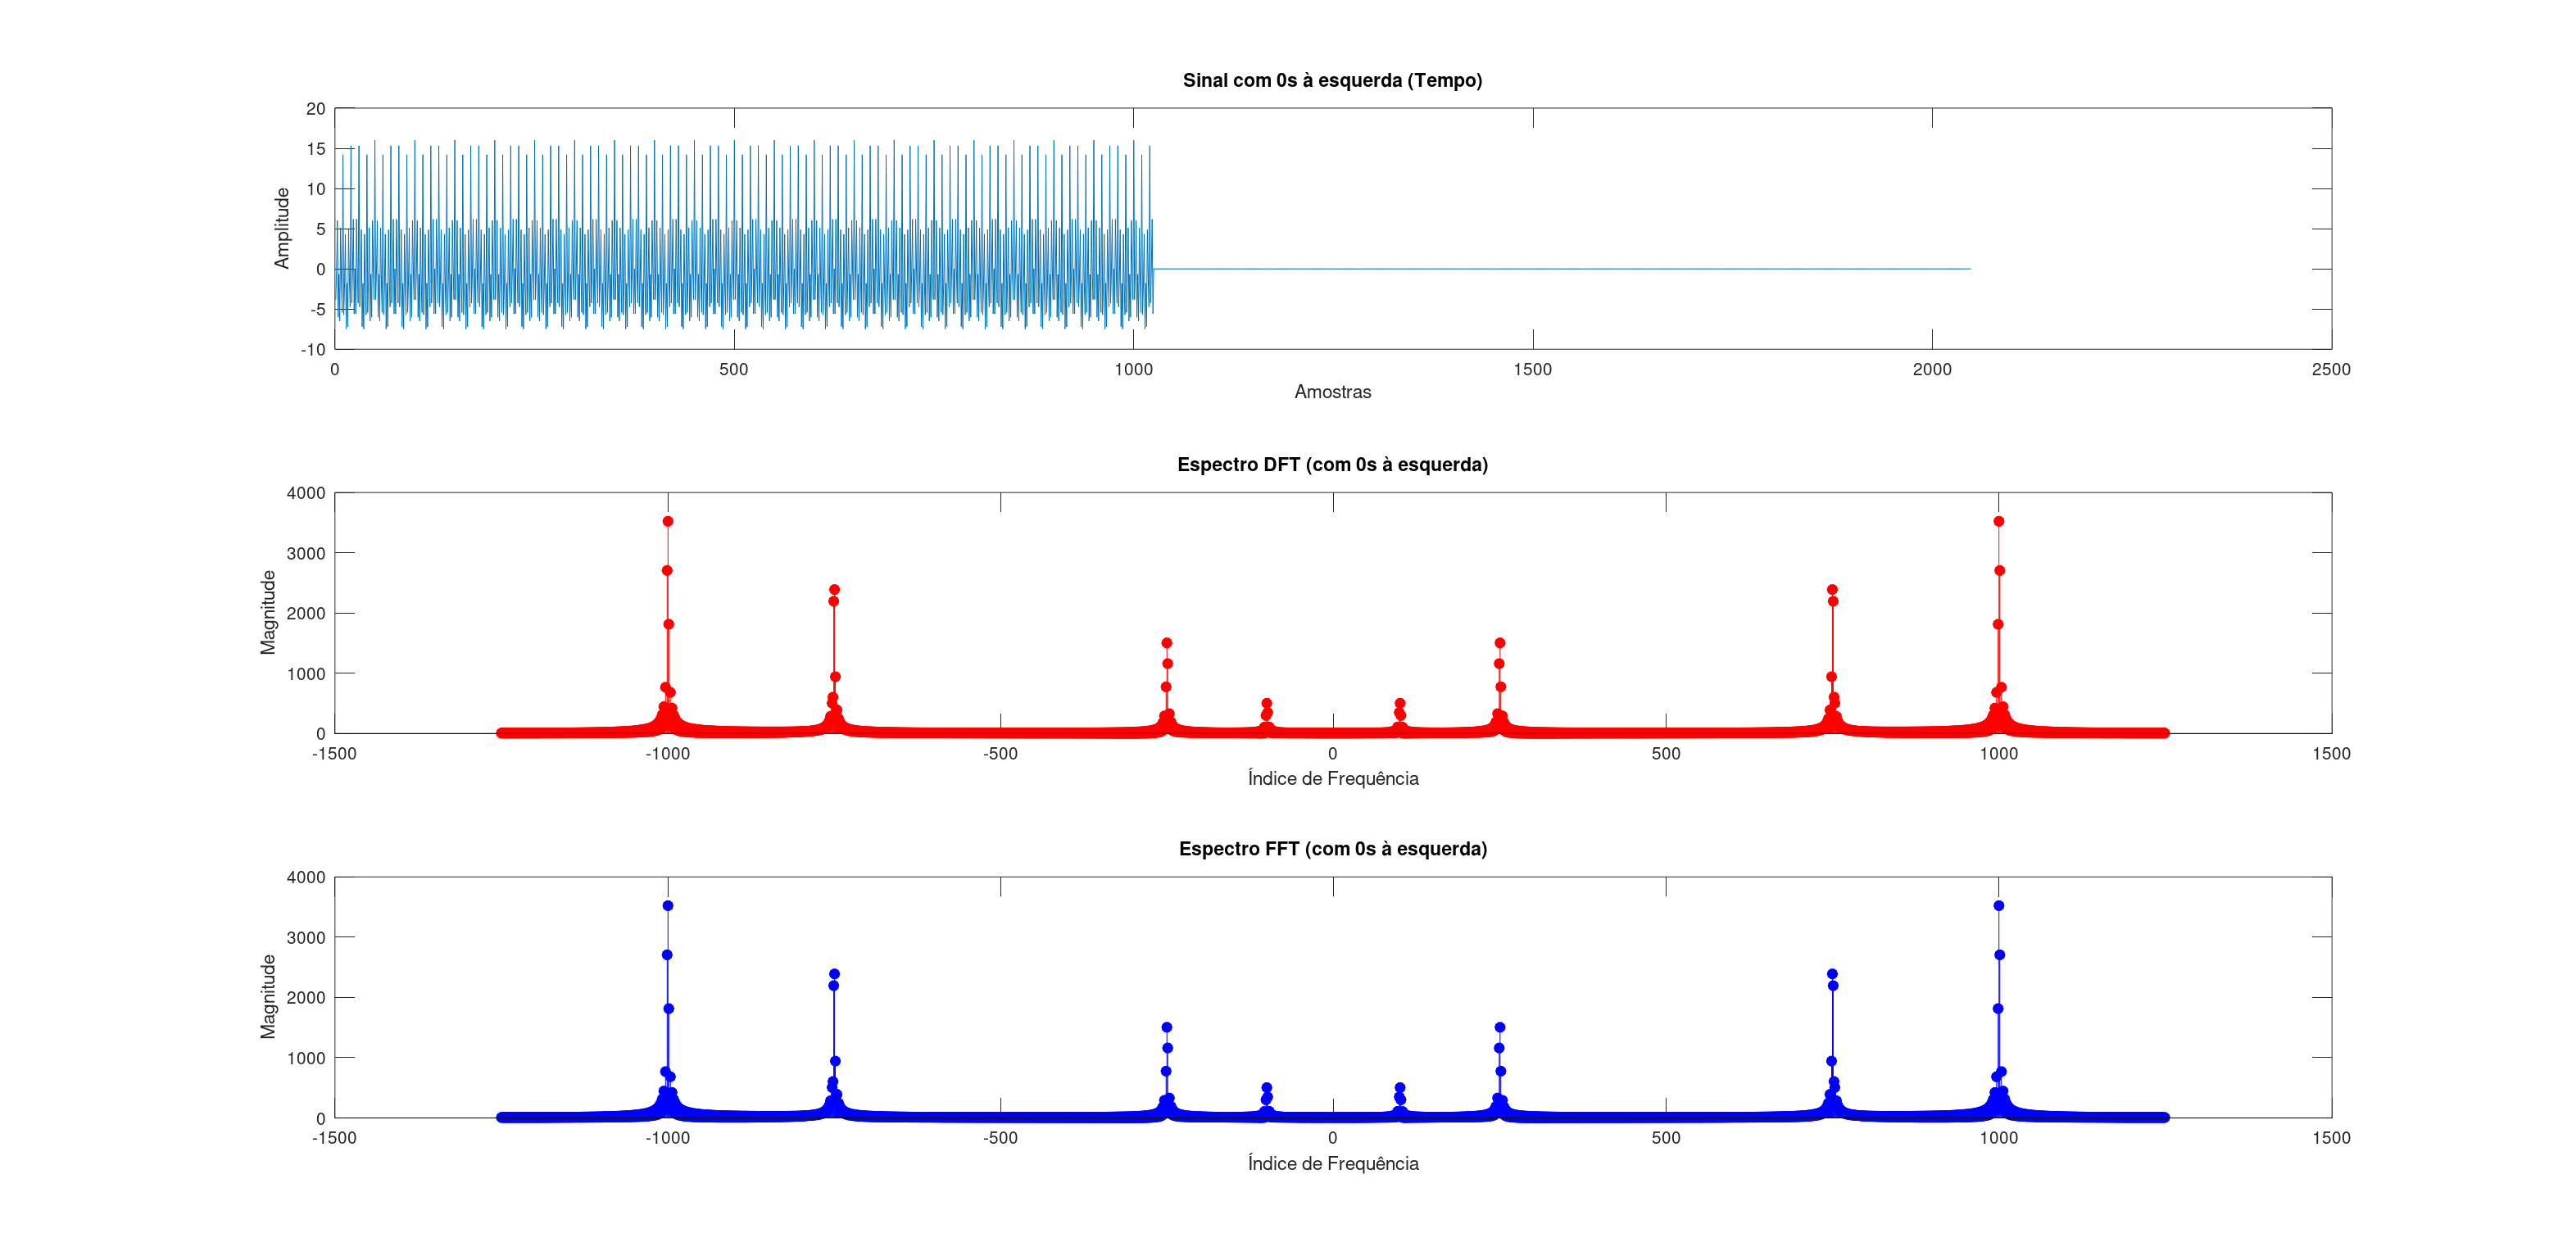
\includegraphics[width=1\linewidth]{03_experimental_analysis//assets/plot_results/1024_samples_dft_fft_padded.png}
    \caption{DFT+FFT Aplicada a 1024 amostras com 1024 zeros à direita}
    \label{fig:signal_1024samples_fft-dft_padded}
\end{figure}

%%%%%%%%%%%%%%%%%%%%%%%%%%%%%%%%%%%%%%%%%%%%%%%%%%%%%%%%%%%%%%%%%%%%

Ao comparar as figuras \textbf{\ref{fig:signal_256samples_fft-dft}}, \textbf{\ref{fig:signal_256samples_fft-dft_padded}}, \textbf{\ref{fig:signal_512samples_fft-dft}}, \textbf{\ref{fig:signal_512samples_fft-dft_padded}}, \textbf{\ref{fig:signal_1024samples_fft-dft}}, e \textbf{\ref{fig:signal_1024samples_fft-dft_padded}}, observa-se que,  apesar dos valores incluídos serem zeros à direita, o resultado final acaba sendo mais refinado com relação à discriminação entre as componentes de frequência e melhora a definição do espectro.

Ao aumentar a quantidade de amostras no sinal, a resolução espectral melhora significativamente, o que é observado nas figuras que ilustram a análise do espectro para diferentes números de amostras. Inicialmente, com 256 amostras, o espectro se torna mais resolvido, permitindo a identificação das frequências dominantes de maneira mais precisa. Ao adicionar 256 zeros à sequência, o espectro se aprimora ainda mais, com picos mais definidos e localizados com maior exatidão. Esse comportamento se repete com o aumento do número de amostras.

O comportamento de melhoria do espectro se repete conforme a quantidade de amostras aumenta, resultando em uma representação cada vez mais precisa do sinal.
